\chapter{Machine Learning Operations}
\label{chap:mloper}

\improvement[inline]{Add outline of how ML, DevOps and MLOps fit together}

%--------------------------------------------------------------------------------------------------------------------------------------------
\section{Machine Learning} % 2 pages
\label{sec:ml}

\subsection{Overview}

\info[inline]{Intro to ML} % Definition and basics of ML
Writing programs and developing algorithms to complete specific tasks is a labor intensive task requiring professional programming expertise.
A different approach is to develop generic algorithms that can change behavior by learning.
The field studying these types of algorithms is called machine learning.
Machine learning algorithms learn by applying an optimization algorithm to adjust set of parameters called a model and this process is called training the model \parencite{lecunDeepLearning2015}. % TODO find reference
A simplified machine learning workflow consists of splitting the data into training and test datasets, performing preprocessing separately for each dataset, training the model on the training dataset and finally evaluating the trained model on the test dataset\todo{ref}.  % TODO find reference


% Usefulness of ML
Machine learning is widely used in applications like search, drug design or ad placement and can be also known as data mining or predictive analytics \parencite{domingosFewUsefulThings2012}. Developing machine learning systems, which are systems that are based on machine learning, can be a difficult task. Unlike traditional software development, experiments with both code and data as inputs are central to machine learning development \parencite{zahariaAcceleratingMachineLearning2018} and reproducibility of the experiments is often problematic. While plenty of research focuses on machine learning methods or even datasets and data quality, the biggest bottleneck is human cycles \parencite{domingosFewUsefulThings2012}. Faster iterations improve the machine learning developer or researcher experience. An important metric to pay attention to and optimize is the mean iteration cycle for machine learning developers.

\info[inline]{Types of ML} % Types of ML
Machine learning can be practiced with two different goals in mind. First is explanatory modeling with the purpose of scientific theory building and testing and the second is predictive modeling mostly used outside of scientific research \parencite{shmueliExplainPredict2010a}.
One practical difference is that unlike predictive modeling, explanatory modeling rarely uses holdout test sets or cross validation for evaluation \parencite{shmueliExplainPredict2010a}.
Lack or presence of evaluation on a test set can be used as a heuristic to quickly determine whether a machine learning project is explanatory or predictive in nature.
However, even explanatory modeling benefits from evaluating the predictive power \parencite{shmueliExplainPredict2010a}.
Domingos \parencite*{domingosFewUsefulThings2012} in their paper assume all machine learning is predictive in nature and state the following:
\begin{quote}
    The fundamental goal of machine learning is to generalize beyond the examples in the training set.
\end{quote}
It is important to keep in mind the end goals of a machine learning project, because common practices in a research setting might not be applicable when creating machine learning systems.

Machine learning algorithms can be categorized as supervised learning, unsupervised learning or reinforcement learning\todo{ref}. %TODO find reference
The main differences are related to whether the model learns by using "right answers" provided by labeled data in supervised learning, by finding structure in the dataset in unsupervised learning or by interacting with the world in reinforcement learning\todo{ref}. %TODO find reference
Model evaluation is also different with supervised learning mostly relying on universal cross-validation on previously unseen data and unsupervised or reinforcement learning relying on internal evaluation metrics tied to the specific algorithm\todo{ref}. %TODO find reference  
Unsupervised learning has the advantage of not requiring labeled data which is an advantage for problems where labels are uncommon \parencite{leBuildingHighlevelFeatures2012}.

\info[inline]{Practical problems}

\subsection{Machine learning performance metrics}
\label{sec:mlperf}
\info[inline]{Intro}
\info[inline]{Training vs Validation metrics}
\info[inline]{Domain specific metrics}


\subsection{Hyperparameter optimization}

\info[inline]{Intro}
% Hyperparameter definition and examples

Parameters given as part of a configuration to the machine learning model are called hyperparameters \parencite{yangHyperparameterOptimizationMachine2020}.
For example learning rate, batch size or a classification threshold are hyperparameters set before the model is trained.
\todo{ref} Most common hyperparameter selection technique in practice is manually adjusting the hyperparameters and is humorously called graduate student descent\todo{ref}. % TODO find reference

% Benefits of hyperparameter search
Automatic tuning of hyperparameters can help achieve state-of-the-art performance in machine learning systems \parencite{maclaurinGradientbasedHyperparameterOptimization2015}.
Hyperparameter optimization techniques include grid search, random search, gradient based optimization and Bayesian optimization and they have different benefits and limitations \parencite{yangHyperparameterOptimizationMachine2020}.

Similar concepts to hyperparameter optimization are neural architecture optimization and meta modeling where model structure or modeling algorithm is treated as a tunable parameter \parencite{bakerAcceleratingNeuralArchitecture2017}.
For example a machine learning system can automate the choosing of the number of neural network layers, the type of layers or even the type of machine learning algorithm.
Tuning hyperparameters is generally a difficult task \parencite{maclaurinGradientbasedHyperparameterOptimization2015}.

\info[inline]{Practical problems}

Traditional hyperparameter tuning methods such as Bayesian optimization are unfeasible for more than 10-20 hyperparameters \parencite{maclaurinGradientbasedHyperparameterOptimization2015}.
More advanced techniques are required if a larger amount of tunable hyperparameters is desired.
Performance prediction is an important step to reduce the amount of computation required for neural architecture search and hyperparameter optimization \parencite{bakerAcceleratingNeuralArchitecture2017}.

\info[inline]{Optimizing hyperparameter search}

\info[inline]{Early stopping}

Early stopping is a technique in which model training is halted before completion\todo{ref}. %TODO find reference
This is done to save on computational resources and the main reason for early stopping is predicting that the model will have poor performance\todo{ref}. %TODO find reference.
Performance prediction usually relies on predicting a machine learning performance metric such as RMSE or F1 score given the current model is performing during training compared to other models\todo{ref}. %TODO find reference

%--------------------------------------------------------------------------------------------------------------------------------------------
\section{DevOps} % 2 pages
\label{sec:devops}

\subsection{Overview}

\info[inline]{Intro to DevOps}
%TODO 1. Intro to DevOps and definition mishra2020, waller2015
% Common interpretation of devops is...
Most common interpretation of DevOps is a focus on software quality, collaboration between development and operations, process speed and rapid feedback \parencite{mishraDevOpsSoftwareQuality2020,wallerIncludingPerformanceBenchmarks2015, pereraImproveSoftwareQuality2017}. The exact definition is problematic as there is no consensus \parencite{smedsDevOpsDefinitionPerceived2015}. DevOps can be viewed from different points of view such as culture, collaboration, automation, measurements and monitoring \parencite{mishraDevOpsSoftwareQuality2020, wallerIncludingPerformanceBenchmarks2015}.

% TODO 2. 


Continuous integration, continuous deployment and continuous monitoring are well known practices in DevOps \parencite{wallerIncludingPerformanceBenchmarks2015} describing the automatic nature of integrating, deploying and monitoring code changes. Performance profiling and monitoring are similar activities and the main difference is whether it's done during the development process or during operations respectively \parencite{wallerIncludingPerformanceBenchmarks2015}. DevOps bridges the gap between evaluating performance during the development process and during operations \parencite{brunnertPerformanceorientedDevOpsResearch2015}.

TODO Devops lifecycle steps

%\begin{figure}[h]
%    \centering
%    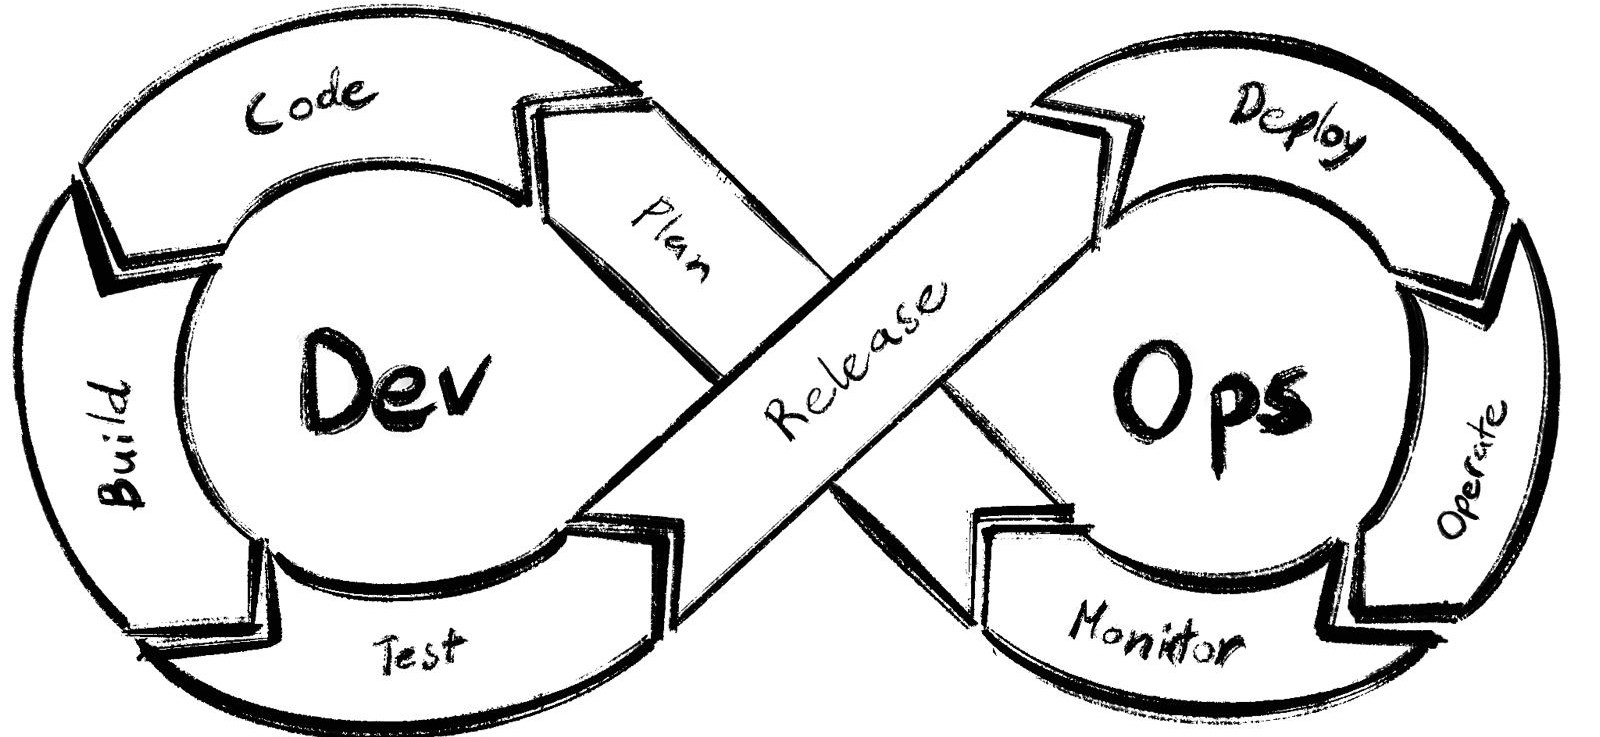
\includegraphics[width=0.75\textwidth]{devops.jpg}
%    \caption{Example of a typical DevOps lifecycle}
%    \label{fig:devops}
%\end{figure}
%

\info[inline]{Practical problems}

TODO resource allocation/resource consumption, small memory software, benchmarking

\subsection{System performance metrics}

\info[inline]{Intro}
Performance metrics are fundamental to all activities involving performance evaluation such as profiling or monitoring \parencite{brunnertPerformanceorientedDevOpsResearch2015}. Common metrics involve measuring the CPU, but other metrics such as memory usage, network traffic or I/O usage are not as well defined as a CPU metric \parencite{brunnertPerformanceorientedDevOpsResearch2015}.

\begin{itemize}
    \item Task Completion time
    \item Throughput
    \item Latency
    \item CPU usage
    \item GPU usage
    \item RAM usage
    \item VRAM usage
    \item I/O usage
    \item Network traffic
\end{itemize}

\info[inline]{System metrics}
\info[inline]{Domain specific metrics}

\subsection{Continuous monitoring and benchmarking}

\info[inline]{Intro}
Preprocessing

Training

Serving Latency

\info[inline]{Practical problems}
Resource demands might change depending on the inputs \parencite{brunnertPerformanceorientedDevOpsResearch2015} making it important to systematically measure performance not only based on code changes but also on configuration changes or even data changes.

\info[inline]{Continuous benchmarking}

%--------------------------------------------------------------------------------------------------------------------------------------------
\section{MLOps} % 4 pages
\label{sec:mldevops}

\subsection{Overview}

TODO \parencite{kreuzbergerMachineLearningOperations2023} data scientists doing manual work issue from conclusions, definition of MLOps, limit to technical stuff and tooling

%TODO rajaa devops teknisiin asioihin
Requirements for a machine learning system are different depending on the task. For example speech and object recognition might have no particular performance requirements during training but has strict latency and computational resource restrictions when deployed to serve large amounts users \parencite{hintonDistillingKnowledgeNeural2015}. One of the key areas of MLOps is using machine learning in production systems in addition to data processing and machine learning model training.

Performance measuring software is not new, but ML brings additional challenges in the form of models and data which requires a modified approach \parencite{breckMLTestScore2017a}. It is also important to note, that not every data scientist or machine learning engineer working on machine learning systems has a software engineering background \parencite{finzerDataScienceEducation2013} and might lack the necessary knowledge to apply software engineering best practices to machine learning systems.

Projects involving machine learning often make common methodological mistakes that threaten the validity of the models, but are easily avoided\todo{ref}. %TODO reference common ml pitfalls paper

TODO MLOps lifecycle steps

\subsection{Machine learning development workflow} \todo{siirretään MLOps osioon}
\label{sec:mlworkflow}


Projects involving machine learning often make common methodological mistakes that threaten the validity of the models, but are easily avoided\todo{ref}. %TODO reference common ml pitfalls paper
Several workflows for developing machine learning systems have emerged attempting to standardize the overall development process including CRISP-DM and KDD\todo{ref}.  %TODO references
These workflows will overall have similar steps. Using CRISP-DM as an example we have the following steps in the workflow: \todo{ref} %TODO crisp-dm, kdd citations

\begin{enumerate}
    \item Business and Data Understanding
    \item Data Preparation
    \item Modeling
    \item Evaluation
    \item Deployment
\end{enumerate}



% TODO CRISP-DM
\todo{ref crisp-dm} Business and Data understanding refers to understanding the problem and the datasets. %TODO crisp-dm

% TODO Data preparation

Preprocessing, feature engineering

% TODO Model training

% TODO Linear regression
% TODO K nearest neighbors
% TODO Neural Network

% TODO Model evaluation

% TODO Model interpretation

%\begin{figure}[h]
%    \centering
%    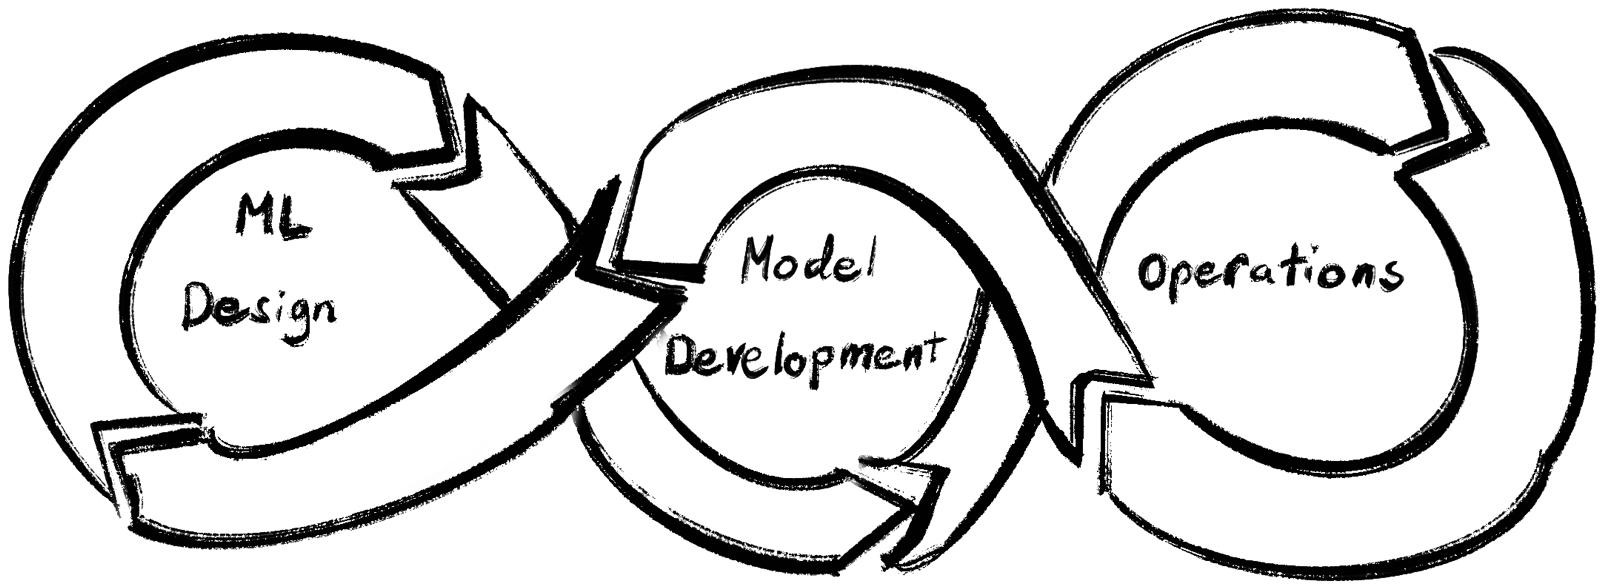
\includegraphics[width=0.75\textwidth]{mlops.jpg}
%    \caption{Example of a typical MLOps lifecycle}
%    \label{fig:mlops}
%\end{figure}

TODO what DevOps brings to ML

TODO Continuous Training

\subsection{AutoML}

Machine learning systems in addition to machine learning performance metrics and system performance metrics will have their performance metrics tied to product or organization metrics such as user churn rate or click-through rate \parencite{shankarOperationalizingMachineLearning2022}. Choosing the right metrics to evaluate a machine learning system is important and the metrics will be different for different machine learning systems \parencite{shankarOperationalizingMachineLearning2022}.

Automated Machine Learning (AutoML) aims to minimize human intervention in completing data analytics tasks using machine learning algorithms \parencite{yangIoTDataAnalytics2022}.

\subsection{Performance prediction and early stopping}

